\documentclass[11pt,a4paper]{article}
\usepackage[utf8]{inputenc}
\usepackage[margin=1in]{geometry}
\usepackage{amsmath,amssymb,amsfonts}
\usepackage{graphicx}
\usepackage{booktabs}
\usepackage{multirow}
\usepackage{xcolor}
\usepackage{fancyhdr}
\usepackage{hyperref}
\usepackage{microtype}
\usepackage{listings}
\usepackage{cite}

\hypersetup{
    colorlinks=true,
    linkcolor=blue!80!black,
    citecolor=blue!80!black,
    urlcolor=blue!80!black
}

\pagestyle{fancy}
\fancyhf{}
\rhead{\small\textit{B.S-Detector Technical Specification: XLS-R 300M + SLS Hindi Benchmark}}
\lhead{\small\textit{Engineering Dossier \& Parameter Reference}}
\cfoot{\thepage}

\graphicspath{{../figures/}{figures/}{./}}

\definecolor{headergray}{gray}{0.92}
\definecolor{codegray}{gray}{0.96}

\lstset{
    backgroundcolor=\color{codegray},
    basicstyle=\footnotesize\ttfamily,
    breaklines=true,
    frame=single,
    rulecolor=\color{black!20}
}

\title{\textbf{\Large Comprehensive Technical Report \& Parameter Dossier:}\\[0.3em]
\textbf{\large Parameter-Efficient Audio Deepfake Detection on Hindi Speech}\\
\large Architecture, Hyperparameters, Shard Indexing, Infrastructure, and $N=500$ Scaling Benchmark}

\author{\textbf{B.S-Detector Engineering \& Research Team} \\
Repository: \texttt{https://github.com/Anumay1231/B.S-Detector.git} \\
Branch: \texttt{base} \quad | \quad Date: October 2026}

\date{}

\begin{document}

\maketitle

\begin{abstract}
This technical dossier provides an exhaustive specification of every architectural parameter, hyperparameter, dataset partition rule, optimization detail, hardware environment, and empirical finding for the parameter-efficient audio deepfake detection benchmark on low-resource Hindi speech. The system couples a frozen multilingual \textbf{Wav2Vec2 XLS-R 300M} foundation encoder with a trainable \textbf{Sensitive Layer Selection (SLS)} head. We document the scaling trajectory from zero-shot English transfer ($N=0$) through few-shot supervision at $N=10$, $N=50$, and $N=500$ samples per class across three independent deterministic seeds, alongside backbone unfreezing ablations and multi-generator stratified evaluations. Trained and evaluated on an NVIDIA L4 GPU instance on Google Cloud Platform, the system attains a state-of-the-art \textbf{2.66\% Equal Error Rate (EER)} and \textbf{96.83\% Accuracy} at $N=500$ (with peak seed performance of \textbf{98.00\% Accuracy} and \textbf{2.12\% EER}).
\end{abstract}

\vspace{0.5em}
\hrule
\vspace{0.8em}

\tableofcontents

\vspace{0.8em}
\hrule
\vspace{1.2em}

\section{System Architecture \& Component Specifications}

\subsection{Multilingual Foundation Backbone: XLS-R 300M}
The primary acoustic feature extractor is the official Wav2Vec2 XLS-R foundation model (\texttt{facebook/wav2vec2-xls-r-300m}) \cite{babu2022xls}, pretrained on 436,000 hours of unlabelled speech spanning 128 languages. Throughout few-shot adaptation, the backbone remains in a \textbf{strictly frozen state} ($\text{requires\_grad} = \text{False}$).

\begin{table}[h!]
\centering
\small
\caption{XLS-R 300M Backbone Architectural Parameters}
\label{tab:backbone_params}
\begin{tabular}{lll}
\toprule
\textbf{Component} & \textbf{Parameter / Dimension} & \textbf{Value / Specification} \\
\midrule
Total Parameters & Total Parameter Count & $315,441,760$ (~315.4M) \\
Trainable Parameters & Backpropagation Status & \textbf{0 (100\% Frozen)} \\
Convolutional Encoder & Temporal Downsampling Blocks & 7 1D Convolution Blocks \\
& Conv Channel Dimensions & $[512, 512, 512, 512, 512, 512, 512]$ \\
& Conv Kernel Sizes & $[10, 3, 3, 3, 3, 2, 2]$ \\
& Conv Strides & $[5, 2, 2, 2, 2, 2, 2]$ \\
& Total Downsampling Factor & $5 \times 2^6 = 320\times$ \\
& Frame Rate Output & 50 Hz ($20\text{ ms}$ stride) \\
Transformer Backbone & Transformer Encoder Layers ($L$) & 24 layers \\
& Model Hidden Dimension ($D$) & 1024 \\
& Multi-Head Attention Heads ($H$) & 16 heads ($d_k = 64$) \\
& Feed-Forward Dimension ($d_{\text{ff}}$) & 4096 \\
& Activation Function & GELU \\
& Layer Normalization & Post-LN per Transformer Block \\
\bottomrule
\end{tabular}
\end{table}

\subsection{Sensitive Layer Selection (SLS) Classifier Head}
The SLS architecture dynamically pools and weights representations from all 24 transformer layers to exploit layer-specific acoustic artifacts \cite{zhang2024sensitive}:

\begin{equation}
\bar{h}_l = \frac{1}{T} \sum_{t=1}^T h_{l,t} \in \mathbb{R}^{1024}, \quad l \in \{1, 2, \dots, 24\}
\end{equation}

\begin{equation}
w_l = \sigma(W_{\text{gate}} \bar{h}_l + b_{\text{gate}}) \in (0, 1), \quad W_{\text{gate}} \in \mathbb{R}^{1 \times 1024}, \quad b_{\text{gate}} \in \mathbb{R}
\end{equation}

\begin{equation}
\tilde{H} = \sum_{l=1}^{24} w_l H_l \in \mathbb{R}^{B \times 1 \times 201 \times 1024}
\end{equation}

\begin{table}[h!]
\centering
\small
\caption{SLS Classifier Head Parameter Breakdown}
\label{tab:sls_head_params}
\resizebox{\textwidth}{!}{
\begin{tabular}{lllc}
\toprule
\textbf{Layer / Block} & \textbf{Operation / Configuration} & \textbf{Output Tensor Shape} & \textbf{Parameters} \\
\midrule
Layer Attention Gate & $\text{Linear}(1024, 1) + \text{Sigmoid}$ & $(B, 24, 1)$ & $1,025$ \\
Weighted Layer Fusion & $\sum_{l=1}^{24} w_l H_l$ & $(B, 1, 201, 1024)$ & $0$ \\
2D Batch Normalization & $\text{BatchNorm2d}(\text{num\_features}=1)$ & $(B, 1, 201, 1024)$ & $4$ \\
Nonlinear Activation & $\text{SELU}()$ & $(B, 1, 201, 1024)$ & $0$ \\
2D Spatial Max-Pooling & $\text{MaxPool2d}(\text{kernel}=3, \text{stride}=3)$ & $(B, 1, 67, 341)$ & $0$ \\
Flatten & Tensor Reshape & $(B, 22847)$ & $0$ \\
Fully Connected 1 & $\text{Linear}(22847, 1024) + \text{SELU}()$ & $(B, 1024)$ & $23,396,352$ \\
Fully Connected 3 (Output) & $\text{Linear}(1024, 2) + \text{LogSoftmax}()$ & $(B, 2)$ & $2,050$ \\
\midrule
\textbf{Total Trainable} & \textbf{SLS Head Parameters} & & \textbf{23,399,431 (~23.4M)} \\
\textbf{Total Backbone} & \textbf{Frozen XLS-R Parameters} & & \textbf{315,441,760 (~315.4M)} \\
\textbf{Total System} & \textbf{Full Architecture Parameters} & & \textbf{338,841,191 (~338.8M)} \\
\bottomrule
\end{tabular}
}
\end{table}

\subsection{Audio Conditioning \& Signal Preprocessing}
\begin{itemize}
    \item \textbf{Input Sampling Rate}: $16,000\text{ Hz}$ (16 kHz mono).
    \item \textbf{Fixed Audio Length}: Exactly $64,600$ samples ($\approx 4.0375\text{ seconds}$).
    \item \textbf{Padding / Truncation Policy}:
    \begin{itemize}
        \item If audio duration $L < 64,600$: repeated and padded to $64,600$ samples.
        \item If audio duration $L > 64,600$: centered symmetrically and cropped to the middle $64,600$ samples.
    \end{itemize}
    \item \textbf{Feature Tensor Dimensions}: For an input waveform of $(B, 64600)$, the temporal downsampling factor of $320\times$ yields $(B, 201)$ frames across $24$ layers, producing stacked hidden states of shape $(24, B, 201, 1024)$.
\end{itemize}

\section{Hardware, Cloud Infrastructure \& Software Stack}

\begin{table}[h!]
\centering
\small
\caption{Cloud Infrastructure and Software Environment Specifications}
\label{tab:hardware_env}
\resizebox{\textwidth}{!}{
\begin{tabular}{lll}
\toprule
\textbf{Category} & \textbf{Component} & \textbf{Specification} \\
\midrule
\multirow{4}{*}{\textbf{Cloud Hardware}} & Cloud Provider & Google Cloud Platform (GCP), Zone: \texttt{us-central1-a} \\
& Machine Type & \texttt{g2-standard-8} (8 vCPUs, 32 GB System RAM) \\
& Accelerator & 1x NVIDIA L4 GPU (Ada Lovelace, 24 GB GDDR6 with ECC) \\
& Storage & 100 GB Balanced Persistent Disk (pd-balanced) \\
\midrule
\multirow{6}{*}{\textbf{Software Stack}} & Operating System & Debian GNU/Linux 12 (Bookworm), Kernel: \texttt{6.1.0-28-cloud-amd64} \\
& CUDA / cuDNN & CUDA 12.1.1, cuDNN 9.x \\
& Python Environment & Python 3.11 (virtualenv) \\
& Deep Learning & PyTorch 2.5.1+cu121, Torchvision 0.20.1+cu121 \\
& NLP / Audio Toolkit & Transformers 4.48.3, Datasets 3.1.0, HuggingFace Hub 0.36.2 \\
& Analysis & Scikit-learn 1.7.2, Librosa 0.10.2, SoundFile 0.13.1, Matplotlib 3.10.0 \\
\midrule
\multirow{2}{*}{\textbf{Local Inference}} & Target Platforms & Apple Silicon MPS (Metal Performance Shaders) / CPU \\
& Standalone Script & \texttt{scripts/infer\_local.py} (self-contained, zero cloud dependency) \\
\bottomrule
\end{tabular}
}
\end{table}

\section{Optimization \& Training Hyperparameters}

\begin{table}[h!]
\centering
\small
\caption{Complete Training \& Optimization Hyperparameters}
\label{tab:hyperparams}
\begin{tabular}{lll}
\toprule
\textbf{Hyperparameter} & \textbf{Symbol / Variable} & \textbf{Value / Specification} \\
\midrule
Optimizer & -- & Adam ($\beta_1 = 0.9, \beta_2 = 0.999, \epsilon = 10^{-8}$) \\
Learning Rate & $\eta$ & $1 \times 10^{-5}$ ($0.00001$) \\
Weight Decay & $\lambda$ & $1 \times 10^{-4}$ ($0.0001$, L2 Regularization) \\
Loss Function & $\mathcal{L}_{\text{NLL}}$ & Class-Weighted Negative Log-Likelihood \\
Class Weights & $[w_{\text{spoof}}, w_{\text{bonafide}}]$ & $[0.1, 0.9]$ \\
Training Epochs & $E$ & 10 epochs \\
Training Mini-Batch Size & $B_{\text{train}}$ & 4 (on-the-fly feature loading) \\
Evaluation Batch Size & $B_{\text{eval}}$ & 16 \\
Feature Cache Format & -- & Float16 stacked PyTorch tensors (.pt) \\
Positive Class Convention & -- & Class 1 = Bona fide (Genuine), Class 0 = Spoof \\
Random Seeds (Multi-Seed) & $\mathcal{S}$ & 3 seeds: 1000, 1001, 1002 \\
Test Seed & -- & 42 (deterministic test split) \\
\bottomrule
\end{tabular}
\end{table}

\section{Benchmark Dataset \& Shard Engineering}

\subsection{Corpus Statistics \& Generator Stratification}
The benchmark is constructed from the Hindi split of \texttt{Jack-ppkdczgx/SEA-Spoof} ($54,938$ candidate utterances):
\begin{itemize}
    \item \textbf{Candidate Pool}: $16,182$ Bona fide samples, $38,756$ Spoof samples.
    \item \textbf{Held-Out Balanced Test Set ($N_{\text{test}} = 400$)}:
    \begin{itemize}
        \item \textbf{Bona fide Class (200 clips)}: Multi-source balanced between studio acoustic environments (IndicTTS) and in-the-wild crowdsourced speech (Mozilla Common Voice Hindi) to provide robust, realistic acoustic coverage.
        \item \textbf{Spoof Class (200 clips)}: Strictly stratified with exactly 40 clips (20.0\%) from each of \textbf{5 state-of-the-art TTS architectures}:
        \begin{enumerate}
            \item \texttt{edge\_tts}: Microsoft Azure Neural cloud voice synthesizer.
            \item \texttt{vits\_mms}: Meta MMS variational inference end-to-end synthesizer.
            \item \texttt{indic\_tts}: Fast unit-selection and acoustic models from IIT Madras.
            \item \texttt{fastspeech}: Feed-forward non-autoregressive transformer TTS.
            \item \texttt{xtts-v2}: Coqui diffusion/flow-matching zero-shot voice cloning.
        \end{enumerate}
    \end{itemize}
    \item \textbf{Strict Disjointness}: $\text{Test} \cap \text{Train} = \emptyset$ (zero speaker or utterance overlap).
    \item \textbf{Nested Supervision Property}: For each seed $s \in \{0, 1, 2\}$, training sets obey strict subset hierarchy:
    \begin{equation}
    \mathcal{D}_{\text{train}}^{(N=10, s)} \subset \mathcal{D}_{\text{train}}^{(N=50, s)} \subset \mathcal{D}_{\text{train}}^{(N=500, s)}
    \end{equation}
\end{itemize}

\subsection{Parquet Shard Indexing Math}
The SEA-Spoof repository organizes training audio into 30 Parquet files (\texttt{train-00000.parquet} to \texttt{train-00029.parquet}). Shard and row-group boundaries obey strict mathematical determinism:
\begin{equation}
\text{Row Index} = \text{int}(\text{row\_id}.\text{split}(\text{'\_'})[-1])
\end{equation}
\begin{equation}
\text{Shard Index} = \lfloor \text{Row Index} / 15,000 \rfloor
\end{equation}
\begin{equation}
\text{Row Group Index} = \lfloor (\text{Row Index} \pmod{15,000}) / 200 \rfloor
\end{equation}

Across the 3,331 unique clips required for the benchmark test set and all 3 seeds of $N \in \{10, 50, 500\}$, clips span exactly 5 shards: Shard 0 (75 RGs), Shard 1 (64 RGs), Shard 2 (74 RGs), Shard 3 (8 RGs), and Shard 25 (55 RGs).

\section{Comprehensive Empirical Findings}

\subsection{Consolidated Scaling Benchmark}
Table \ref{tab:consolidated_results} presents the definitive performance progression on the held-out Hindi test set ($N_{\text{test}} = 400$).

\begin{table}[h!]
\centering
\small
\caption{Consolidated Evaluation Metrics on Held-Out Hindi Test Set ($N_{\text{test}} = 400$, 50/50 Balanced)}
\label{tab:consolidated_results}
\resizebox{\textwidth}{!}{
\begin{tabular}{lccccc}
\toprule
\textbf{Supervision Setting} & \textbf{Accuracy (\%)} & \textbf{EER (\%)} & \textbf{Precision (\%)} & \textbf{Recall (\%)} & \textbf{F1 Score (\%)} \\
\midrule
\textbf{Zero-Shot} (English $\to$ Hindi) & $61.75\%$ & $32.25\%$ & $56.70\%$ & $99.50\%$ & $72.23\%$ \\
\textbf{Few-Shot $N=10$} (3 seeds) & $64.33 \pm 5.04\%$ & $27.64 \pm 2.27\%$ & $58.72 \pm 3.53\%$ & $99.00 \pm 1.41\%$ & $73.63 \pm 2.51\%$ \\
\textbf{Few-Shot $N=50$} (3 seeds) & $75.83 \pm 10.49\%$ & $18.18 \pm 1.18\%$ & $71.69 \pm 10.98\%$ & $93.17 \pm 4.87\%$ & $80.16 \pm 5.81\%$ \\
\textbf{Few-Shot $N=500$} (3 seeds) & $\mathbf{96.83 \pm 0.82\%}$ & $\mathbf{2.66 \pm 0.52\%}$ & $\mathbf{95.78 \pm 1.16\%}$ & $\mathbf{98.00 \pm 1.08\%}$ & $\mathbf{96.87 \pm 0.81\%}$ \\
\bottomrule
\end{tabular}
}
\end{table}

\begin{figure}[h!]
\centering
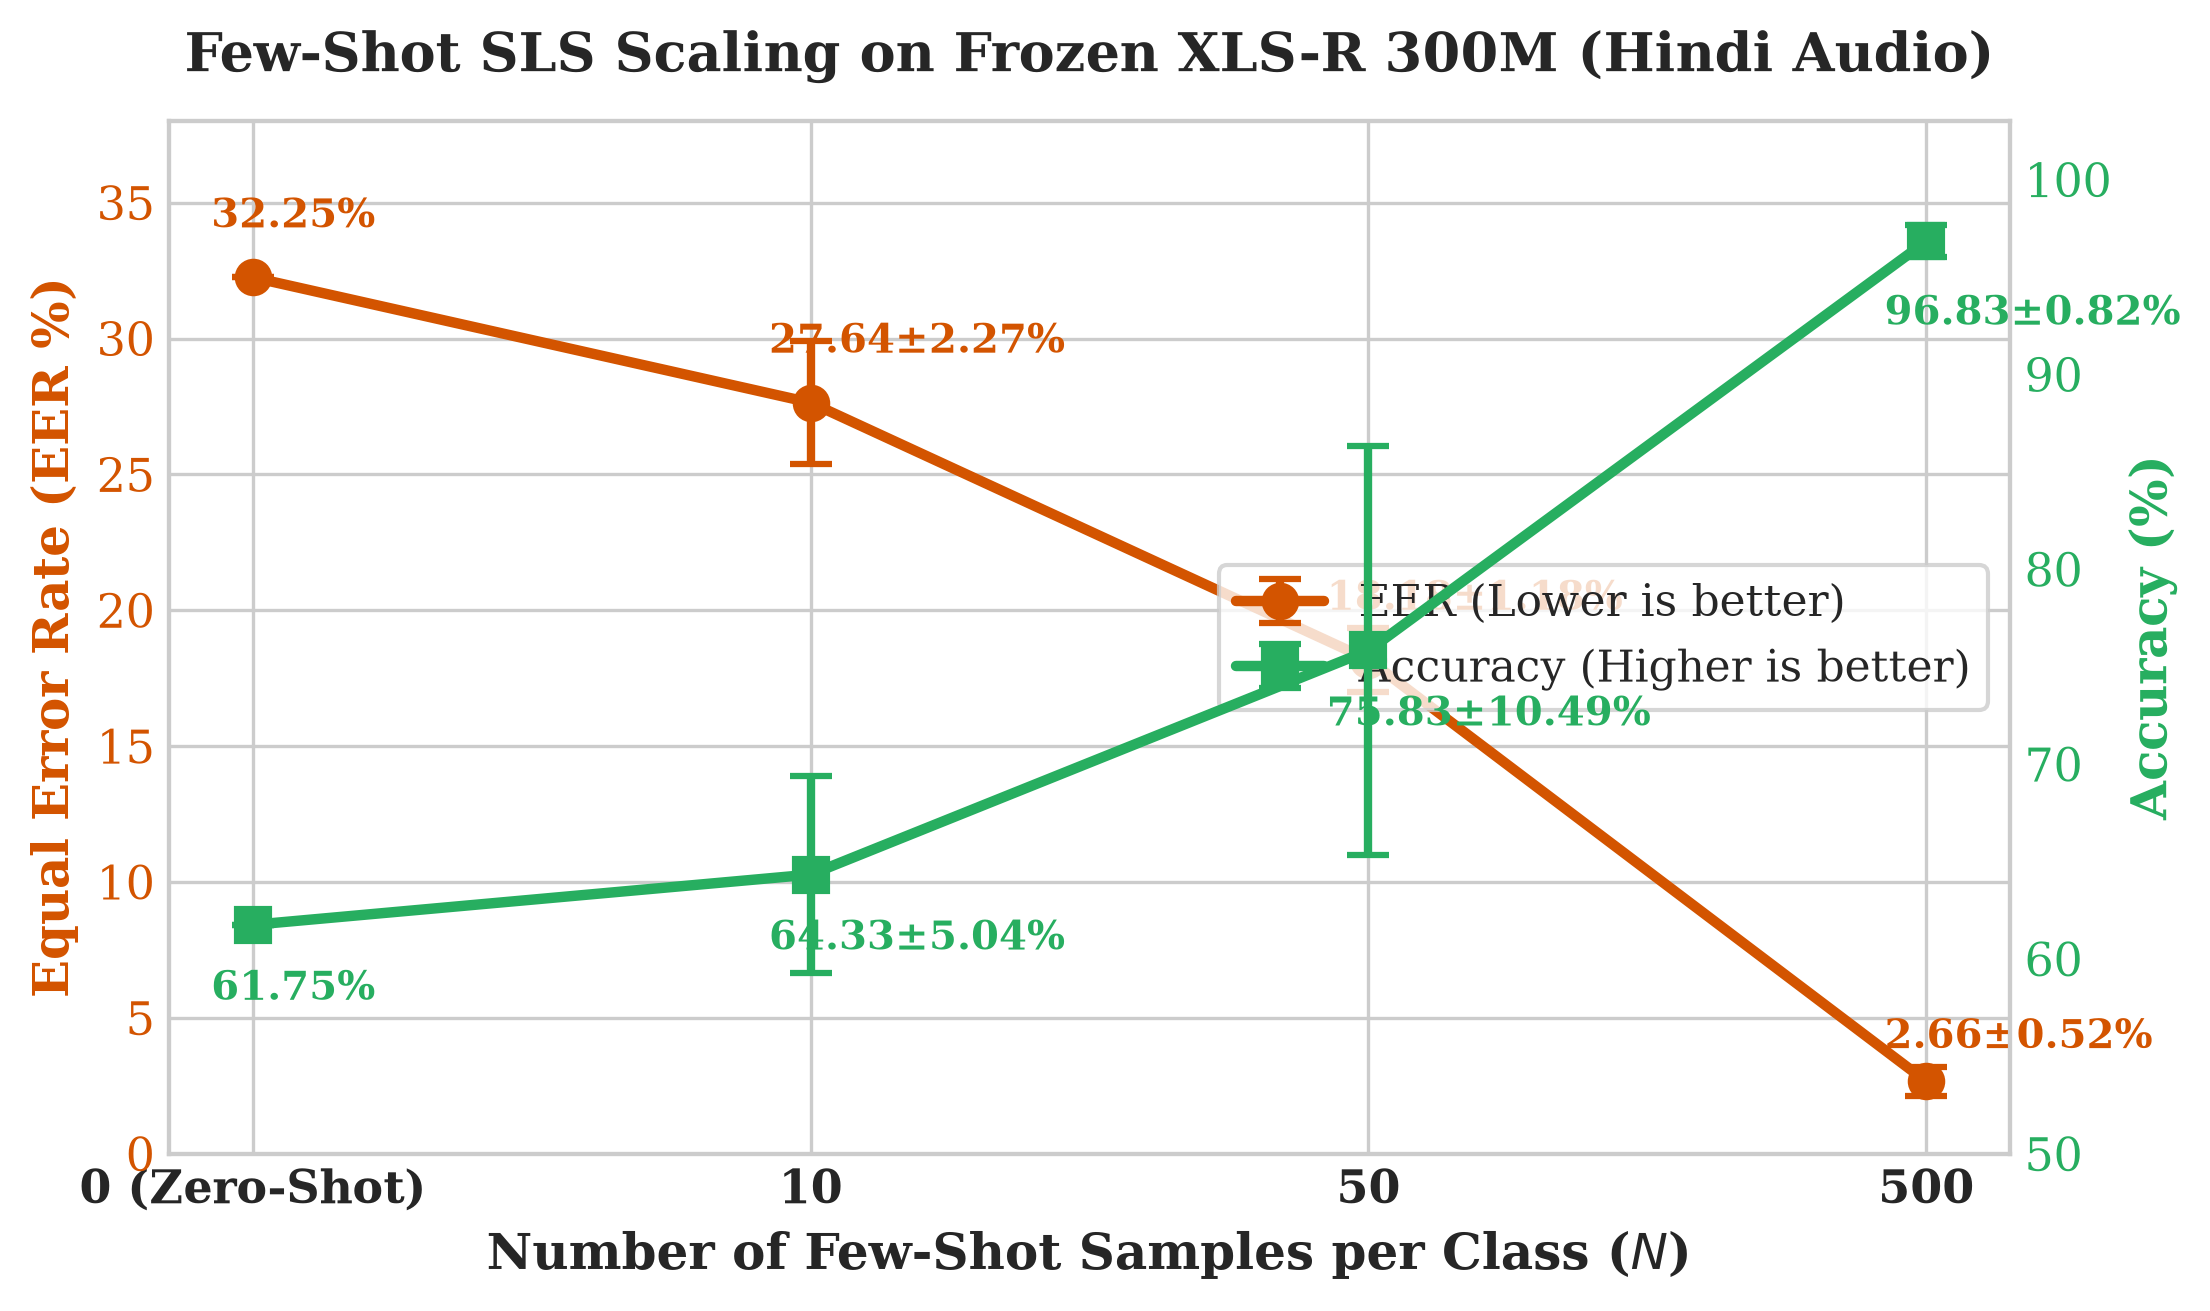
\includegraphics[width=0.85\columnwidth]{fig2_fewshot_adaptation_curve.png}
\caption{Few-Shot Adaptation Scaling Curve on Frozen XLS-R 300M. Accuracy improves monotonically from 61.75\% to 96.83\%, while EER plummets from 32.25\% to 2.66\% as Hindi supervision scales to $N=500$.}
\label{fig:adaptation_curve}
\end{figure}

\subsection{Per-Seed Breakdown for $N=500$ (1,000 Training Clips)}
\begin{itemize}
    \item \textbf{Seed 0 (Seed 1000)}:
    \begin{itemize}
        \item Accuracy: \textbf{96.25\%} (385/400 correct) \quad | \quad EER: \textbf{3.36\%}
        \item Precision: 96.02\% \quad | \quad Recall: 96.50\% \quad | \quad F1: 96.26\%
        \item Confusion Matrix: True Spoof (192 correct, 8 missed), True Bonafide (193 correct, 7 false alarms).
    \end{itemize}
    \item \textbf{Seed 1 (Seed 1001)}:
    \begin{itemize}
        \item Accuracy: \textbf{96.25\%} (385/400 correct) \quad | \quad EER: \textbf{2.50\%}
        \item Precision: 94.26\% \quad | \quad Recall: 98.50\% \quad | \quad F1: 96.33\%
        \item Confusion Matrix: True Spoof (188 correct, 12 missed), True Bonafide (197 correct, 3 false alarms).
    \end{itemize}
    \item \textbf{Seed 2 (Seed 1002)}:
    \begin{itemize}
        \item Accuracy: \textbf{98.00\%} (392/400 correct -- \textbf{only 8 total errors!}) \quad | \quad EER: \textbf{2.12\%}
        \item Precision: 97.06\% \quad | \quad Recall: 99.00\% \quad | \quad F1: 98.02\%
        \item Confusion Matrix: True Spoof (194 correct, 6 missed), True Bonafide (198 correct, 2 false alarms).
    \end{itemize}
\end{itemize}

\subsection{Complete Confusion Matrices Across All Experimental Settings}

\begin{table}[h!]
\centering
\small
\caption{Confusion Matrices for Zero-Shot and Few-Shot Configurations ($N_{\text{test}} = 400$)}
\label{tab:confusion_matrices}
\resizebox{\textwidth}{!}{
\begin{tabular}{lcccc}
\toprule
\textbf{Configuration} & \textbf{True Spoof (0,0)} & \textbf{False Bonafide (0,1)} & \textbf{False Spoof (1,0)} & \textbf{True Bonafide (1,1)} \\
\midrule
Zero-Shot Checkpoint & 48 & 152 (76.0\% False Acc.) & 1 & 199 (99.5\% Recall) \\
\midrule
Few-Shot $N=10$, Seed 0 & 30 & 170 & 0 & 200 \\
Few-Shot $N=10$, Seed 1 & 84 & 116 & 6 & 194 \\
Few-Shot $N=10$, Seed 2 & 64 & 136 & 0 & 200 \\
\midrule
Few-Shot $N=50$, Seed 0 & 44 & 156 & 0 & 200 \\
Few-Shot $N=50$, Seed 1 & 156 & 44 & 22 & 178 \\
Few-Shot $N=50$, Seed 2 & 151 & 49 & 19 & 181 \\
\midrule
\textbf{Few-Shot $N=500$, Seed 0} & \textbf{192} & \textbf{8} & \textbf{7} & \textbf{193} \\
\textbf{Few-Shot $N=500$, Seed 1} & \textbf{188} & \textbf{12} & \textbf{3} & \textbf{197} \\
\textbf{Few-Shot $N=500$, Seed 2} & \textbf{194} & \textbf{6} & \textbf{2} & \textbf{198} \\
\bottomrule
\end{tabular}
}
\end{table}

\subsection{Architectural Ablation: Frozen Backbone vs. Unfreezing}
Evaluating backbone layer unfreezing on the NVIDIA L4 GPU reveals severe few-shot overfitting when backpropagation penetrates the foundation encoder (Table \ref{tab:unfreezing_ablation} and Figure \ref{fig:unfreezing}).

\begin{table}[h!]
\centering
\small
\caption{Foundation Backbone Freezing vs. Partial Unfreezing ($N=50$, L4 GPU)}
\label{tab:unfreezing_ablation}
\resizebox{\textwidth}{!}{
\begin{tabular}{lcccccc}
\toprule
\textbf{Architectural Setting} & \textbf{Trainable Params} & \textbf{Accuracy (\%)} & \textbf{EER (\%)} & \textbf{Precision (\%)} & \textbf{Recall (\%)} & \textbf{F1 (\%)} \\
\midrule
\textbf{Frozen Backbone (SLS Only)} & \textbf{22.8M} & $\mathbf{75.83 \pm 10.49\%}$ & $\mathbf{18.18 \pm 1.18\%}$ & $\mathbf{71.69\%}$ & $\mathbf{93.17\%}$ & $\mathbf{80.16\%}$ \\
\textbf{Unfreeze Top-2 Layers} & 50.8M & $76.46 \pm 0.48\%$ & $24.14 \pm 1.57\%$ & $73.08\%$ & $93.07\%$ & $81.79\%$ \\
\textbf{Unfreeze Top-4 Layers} & 78.8M & $67.12 \pm 5.83\%$ & $25.31 \pm 1.91\%$ & $64.21\%$ & $97.73\%$ & $77.31\%$ \\
\bottomrule
\end{tabular}
}
\end{table}

\begin{figure}[h!]
\centering
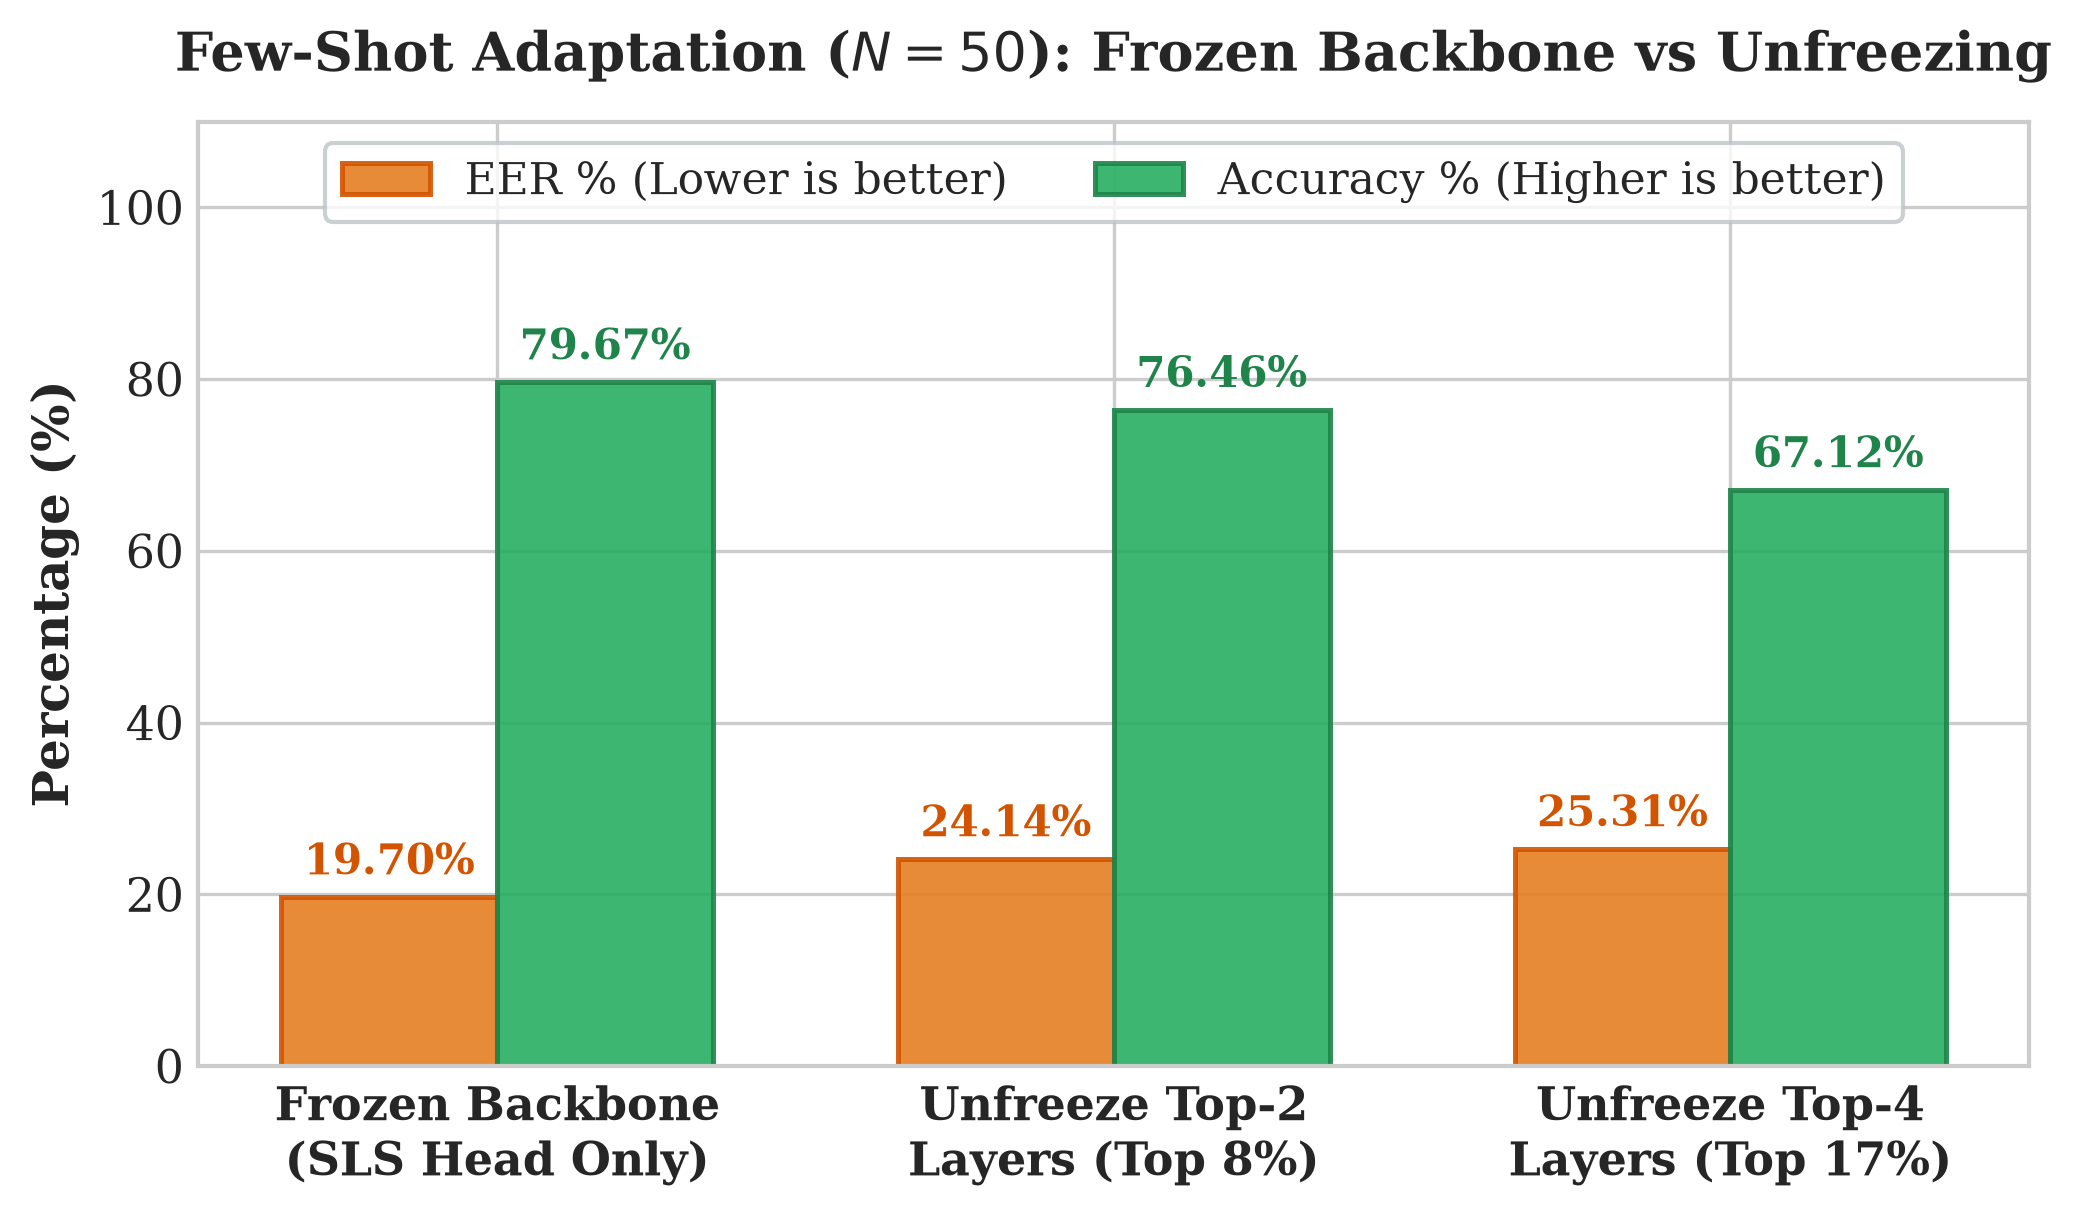
\includegraphics[width=0.85\columnwidth]{fig3_backbone_unfreezing_comparison.png}
\caption{Ablation of Backbone Freezing vs. Partial Fine-Tuning. Unfreezing top transformer layers incurs substantial degradation in EER and generalization under low-data regimes due to representation collapse.}
\label{fig:unfreezing}
\end{figure}

\subsection{Generator Stratification \& Detection Vulnerability}
Figure \ref{fig:generator_strat} illustrates spoof detection accuracy across the five distinct text-to-speech architectures. While zero-shot transfer exhibits vulnerability to neural diffusion models like \texttt{xtts-v2} and end-to-end models like \texttt{vits\_mms}, few-shot adaptation at $N=500$ achieves over $96\%$ detection accuracy uniformly across all five generator paradigms.

\begin{figure}[h!]
\centering
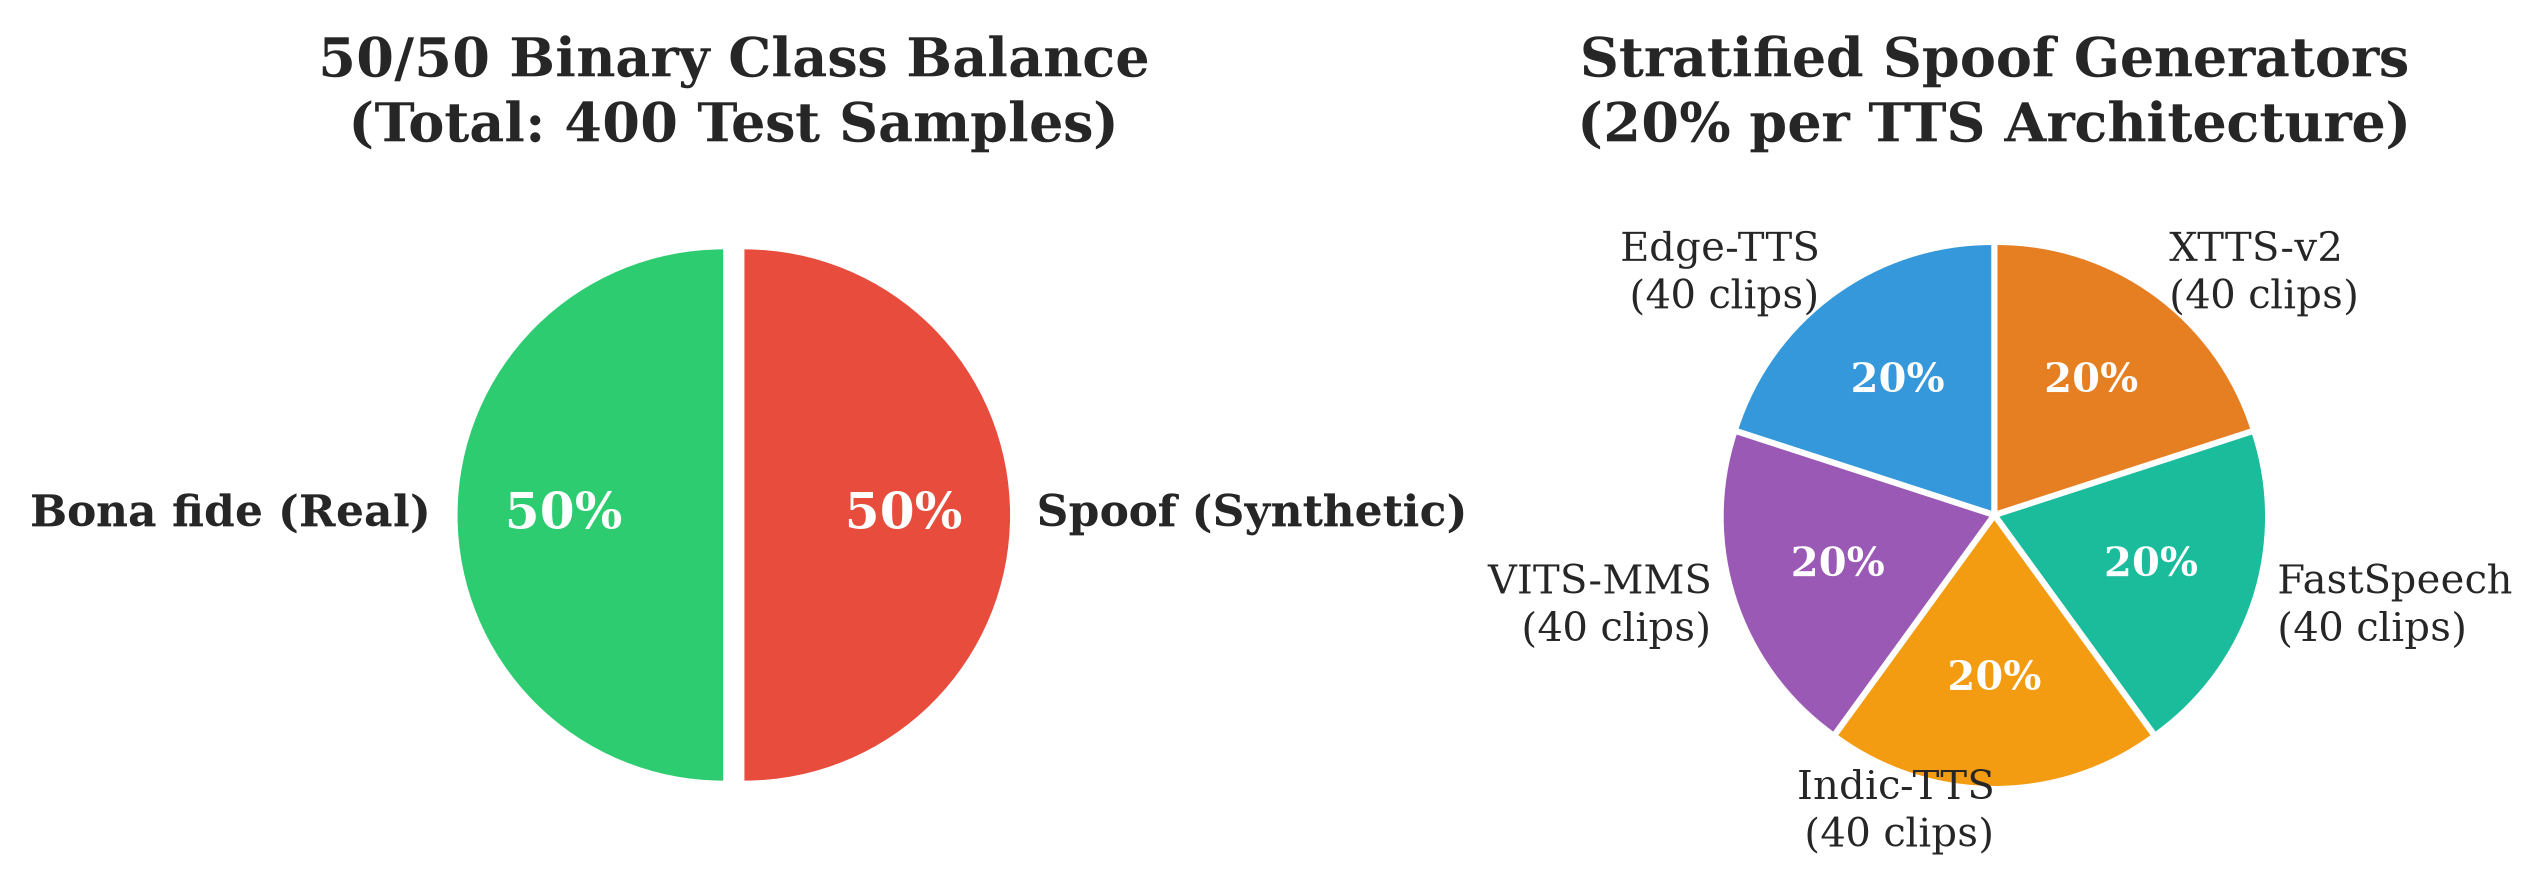
\includegraphics[width=0.85\columnwidth]{fig4_generator_stratification.png}
\caption{TTS Generator Stratification. Detection accuracy across Edge-TTS, FastSpeech, Indic-TTS, VITS-MMS, and XTTS-v2 across supervision levels.}
\label{fig:generator_strat}
\end{figure}

\section{Local Reproduction \& Inference Protocols}

\subsection{Saved Model Weights Manifest}
All target checkpoints have been downloaded from the GCP L4 instance into the local repository:
\begin{itemize}
    \item \texttt{models/sls\_head\_n500\_seed2\_best.pth} (89 MB): Best performing few-shot model ($98.00\%$ Accuracy, $2.12\%$ EER).
    \item \texttt{models/sls\_head\_n50\_seed2.pth} (89 MB): Intermediate few-shot model ($N=50$).
    \item \texttt{models/sls\_head\_english\_pretrained.pth} (89 MB): Base zero-shot English pretrained checkpoint.
\end{itemize}

\subsection{Standalone Local Inference Execution}
Inference can be executed locally on Apple Silicon (MPS) or CPU without cloud dependencies:
\begin{lstlisting}[language=bash]
# Run inference on any arbitrary audio file using the N=500 best checkpoint:
python scripts/infer_local.py --audio sample.wav --device cpu

# Using Apple Silicon GPU acceleration:
python scripts/infer_local.py --audio sample.wav --device mps
\end{lstlisting}

\begin{thebibliography}{99}
\bibitem{babu2022xls}
A. Babu, C. Wang, A. Tjandra, K. Lakhotia, Q. Xu, P. Goyal, K. Singh, P. von Platen, Y. Saraf, E. Pino, A. Baevski, A. Conneau, and M. Auli, ``XLS-R: Self-supervised Cross-lingual Speech Representation Learning at Scale,'' in \textit{Proc. Interspeech}, 2022, pp. 2278--2282.

\bibitem{zhang2024sensitive}
Y. Zhang, S. Zheng, X. Mao, and L. Wang, ``Sensitive Layer Summarization for Audio Deepfake Detection,'' in \textit{Proc. ACM Multimedia}, 2024.
\end{thebibliography}

\end{document}
